\ifx\allfiles\undefined
\documentclass[UTF8]{ctexart}
\title{知识准备}
\author{邹远春}
\date{}
\usepackage{xeCJK}
\usepackage{graphicx, subfig}
\usepackage{caption}
\usepackage{listings}
\usepackage{verbatim}
\begin{document}
\maketitle
\else
\chapter{知识准备}
\fi
\section{RLP}

https://github.com/ethereum/wiki/wiki/RLP

\paragraph{RLP(Recursive Length Prefix)编码}

RLP编码其实提供了一种序列化的编码方法,无论输入是何种嵌套形式的元素或数组,编码输出形式都是[]byte.
RLP是可逆的,它提供了互逆的编码、解码方法。

\subsection{Definition}

\subsection{Examples}

\subsection{RLP~decoding}

以太坊中具体使用的哈希算法,就是对某个类型对象的RLP编码值做了SHA3哈希运算,可称为RLP Hash。以太坊在底层存储中特意选择了专门存储和读取[k,v]键值对的第三方数据库,[k,v]中的v就是某个结构体对象的RLP编码值([]byte),k大多数情况就是v的RLP编码后的SHA-3哈希值。

\section{MPT}

以太坊MPT详解

https://blog.csdn.net/weixin\_41545330/article/details/79370198

\begin{figure}
	\centering
	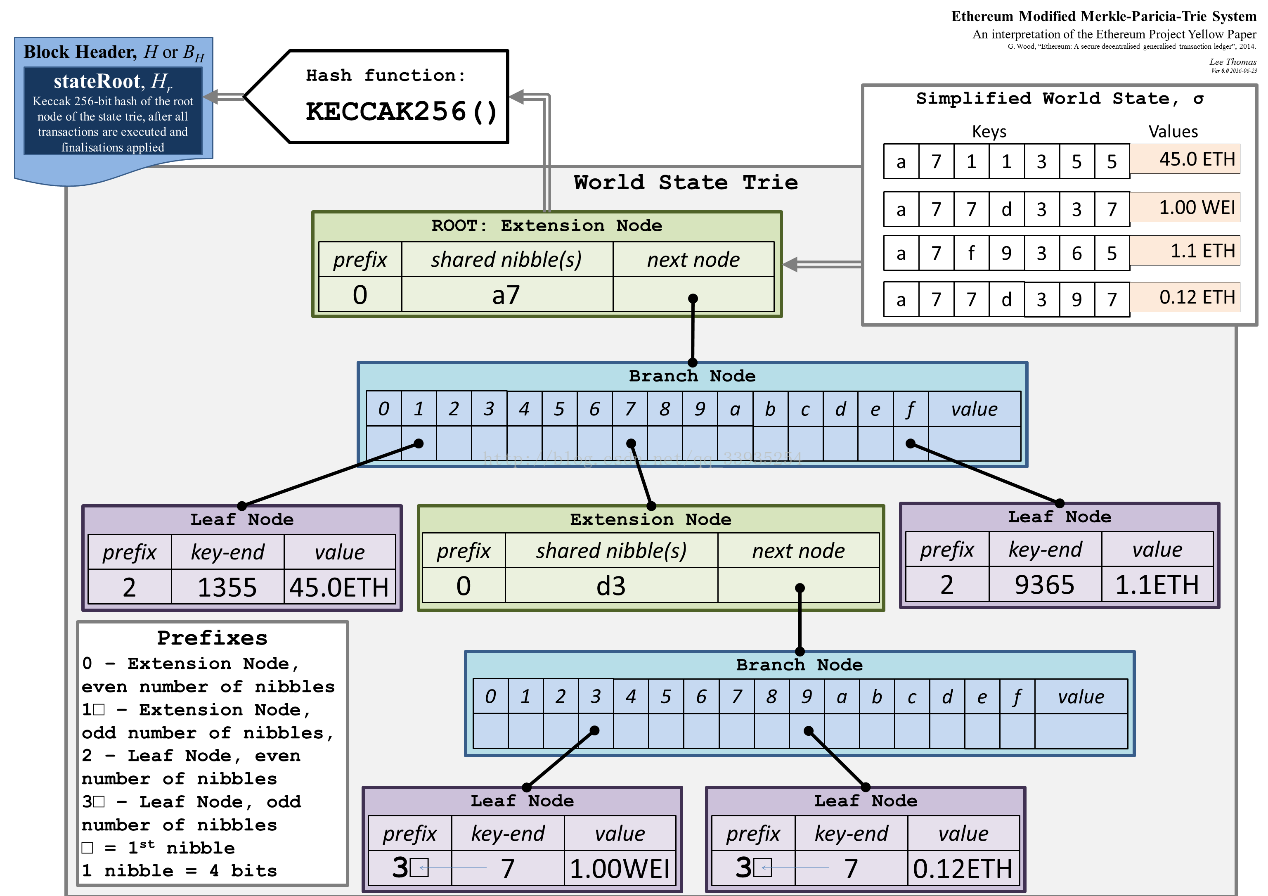
\includegraphics{rlp.png}
	\caption{MTP}
	\label{rlp}
\end{figure}

\section{智能合约1.0}

比特币网络中的交易 https://zhuanlan.zhihu.com/p/33119459

比特币中的脚本系统 https://zhuanlan.zhihu.com/p/33157713

P2PKH
P2PK
多重签名
P2SH

\section{矿池}

\section{矿机}

\section{世界状态}

\section{分叉}

\section{侧链}

RootStock

\section{闪电网络}

\section{隔离见证}

\section{智能合约}

\section{跨链}

\subsection{公证人}
Notary schemes

\subsection{侧链/中继}
Sidechains/relays

BTC-Replay

Cosmos

Polkadot

\subsection{哈希锁定}
Hash-locking

HTLC

\section{预言机Oracle}

\section{Sharding}

\section{中心化交易所}

\section{去中心化交易所}

\section{钱包}

冷钱包就是不联网的钱包,也叫离线钱包。热钱包就是保持联网上线的钱包,也就是热钱包。

硬件钱包。

\subsection{非确定性(随机)钱包}

在最早的一批比特币客户端中,钱包只是随机生成的私钥集合。这种类型的钱包被称作零型非确定钱包。

\subsection{分层确定性钱包}

比特币改进协议BIP32 https://www.jianshu.com/p/d6187961bc35

钱包的技术细节之种子的创建过程 https://zhuanlan.zhihu.com/p/32933727

钱包 精通比特币(第二版) http://book.8btc.com/books/6/masterbitcoin2cn/\_book/ch05.html

\section{ERC20}

\section{ERC721}

\section{安全}
形式化证明

\ifx\allfiles\undefined
\end{document}
\fi